\chapter{Previsão do Prêmio de Risco de Volatilidade com \textit{Machine Learning}}
\label{chap:ml_bvrp}

\section{Motivação e Objetivo do Capítulo}
\label{sec:cap8_motivacao}

Os resultados empíricos apresentados no Capítulo~\ref{chap:estrategias}
indicam que o Prêmio de Risco de Volatilidade do Bitcoin (BVRP) contém informação
relevante para a construção de estratégias condicionais, sobretudo quando o sinal
se encontra em níveis elevados e em ambientes específicos de volatilidade realizada.
Ainda assim, as estratégias avaliadas baseiam-se em regras determinísticas simples,
definidas por limiares fixos e decisões binárias de alocação.

Embora tais abordagens sejam transparentes e economicamente interpretáveis, elas
impõem limitações importantes. Em particular, regras exógenas dificilmente capturam:
(i) interações entre múltiplas variáveis do mercado à vista e de derivativos;
(ii) relações não lineares ou assimétricas; e (iii) variação temporal na relevância
das variáveis explicativas (\textit{state dependence}), típica em mercados com mudanças
frequentes de regime, como o de criptoativos.

Nesse contexto, técnicas de \textit{machine learning} oferecem um arcabouço mais
flexível para modelar a dinâmica do BVRP, permitindo incorporar simultaneamente
múltiplos preditores e estruturas não lineares, sob protocolos de validação temporal
que respeitam o ambiente fora da amostra.

O objetivo deste capítulo é investigar se modelos de \textit{machine learning}
são capazes de prever o BVRP fora da amostra de forma estatisticamente e
economicamente relevante. Para isso, compara-se o desempenho de diferentes classes
de modelos supervisionados sob um desenho experimental rigoroso, incluindo
\textit{benchmarks} fortes baseados na persistência temporal do próprio BVRP.

\section{Formulação do Problema Preditivo}
\label{sec:cap8_problema}

O problema preditivo consiste em estimar o valor futuro do prêmio de risco de
volatilidade em um horizonte $h$, utilizando exclusivamente informação disponível
até o instante $t$. Seja $\text{BVRP}_t$ o prêmio de risco associado a uma janela
padrão (por exemplo, 30 dias), construído como a diferença entre a volatilidade
implícita observada em $t$ e a volatilidade realizada medida ex-post na janela
subsequente. De forma geral:
\begin{equation}
\text{BVRP}_{t} = \text{IV}_{t}^{(30)} - \text{RV}_{t\rightarrow t+30}^{(30)}.
\end{equation}

A tarefa de previsão é definida como:
\begin{equation}
\widehat{\text{BVRP}}_{t+h} = f\left(\mathbf{X}_t\right),
\end{equation}
em que $\mathbf{X}_t$ denota o vetor de variáveis explicativas observadas em $t$,
e $f(\cdot)$ representa a função estimada pelo modelo supervisionado.

Na implementação empírica, utiliza-se tipicamente horizonte curto (por exemplo,
$h=1$ dia), de modo a reproduzir um ambiente realista de decisão e evitar predições
triviais de valores contemporâneos. Em todos os casos, as variáveis são alinhadas
para garantir ausência de \textit{look-ahead bias} e de vazamento de informação
(\textit{data leakage}).

\section{Dados e Variáveis Explicativas}
\label{sec:cap8_dados}

O conjunto de variáveis explicativas incorpora informações do mercado à vista e do
mercado de derivativos de Bitcoin, com ênfase em variáveis associadas à dinâmica de
volatilidade e ao próprio comportamento do prêmio de risco. Em particular, são
consideradas categorias de preditores como:

\begin{itemize}
    \item \textbf{dinâmica dos retornos}: retornos diários e defasagens, além de medidas de
    assimetria e dispersão em janelas móveis (quando disponíveis);
    \item \textbf{dinâmica do prêmio e da volatilidade}: defasagens do BVRP, variações da
    volatilidade implícita e realizada, e diferenças de curto prazo (momentum/reversão);
    \item \textbf{efeitos de calendário}: dummies de dia da semana, mês e/ou feriados relevantes,
    quando apropriado;
    \item \textbf{indicadores de regime}: proxies para estados de baixa/média/alta volatilidade,
    construídos a partir de quantis/tercis da volatilidade realizada (ou métricas análogas).
\end{itemize}

Todas as variáveis são construídas e defasadas de modo consistente, assegurando que
apenas informação disponível no instante $t$ seja utilizada para prever
$\text{BVRP}_{t+h}$. Adicionalmente, variáveis que incorporam diretamente informação
futura (por exemplo, retornos futuros ou volatilidade realizada calculada com dados
posteriores a $t$) são excluídas do conjunto de preditores.

\section{Modelos de \textit{Machine Learning}}
\label{sec:cap8_modelos}

São avaliados algoritmos supervisionados representando diferentes classes de modelos
preditivos, com foco em comparação entre parcimônia, flexibilidade e capacidade de
generalização fora da amostra:

\begin{itemize}
    \item \textbf{Regressões lineares regularizadas}: Ridge ($L_2$) e LASSO ($L_1$),
    que oferecem regularização e seleção implícita de variáveis;
    \item \textbf{Modelos baseados em árvores}: \textit{Random Forests}, capazes de capturar
    interações e não linearidades sem impor forma funcional paramétrica;
    \item \textbf{Métodos de \textit{Gradient Boosting}}: modelos de árvores sequenciais
    (por exemplo, GBRT, XGBoost), que reduzem vieses ao aprender padrões residuais.
\end{itemize}

Os hiperparâmetros são selecionados por validação temporal, com foco no desempenho
fora da amostra e mitigação de sobreajuste.

\section{Desenho Experimental e Avaliação Fora da Amostra}
\label{sec:cap8_oos}

A avaliação do desempenho preditivo é conduzida por meio de um esquema estritamente
fora da amostra, com divisão temporal entre conjuntos de treinamento, validação e
teste, respeitando a ordem cronológica das observações (sem embaralhamento).
O conjunto de validação é utilizado para seleção de hiperparâmetros; o conjunto de
teste é reservado para avaliação final e não participa de escolhas de modelo.

Para interpretar corretamente ganhos preditivos, as previsões são comparadas a
\textit{benchmarks} fortes baseados em persistência temporal do BVRP, como:
(i) \textit{último valor} ($\widehat{\text{BVRP}}_{t+1}=\text{BVRP}_t$) e
(ii) médias móveis de curto prazo. Esses baselines são especialmente relevantes
quando o alvo apresenta alta persistência, o que costuma ocorrer em medidas de
volatilidade e prêmios associados.

O desempenho é avaliado com base em métricas estatísticas como MAE, RMSE/MSE e
$R^2$ fora da amostra. Adicionalmente, discute-se a interpretação econômica e a
viabilidade de incorporar previsões do BVRP em regras de alocação dinâmica.

\section{Resultados Empíricos}
\label{sec:cap8_resultados}

Esta seção apresenta os resultados da previsão do Prêmio de Risco de Volatilidade
do Bitcoin fora da amostra. Inicialmente, reporta-se o desempenho estatístico dos
modelos. Em seguida, discute-se a comparação entre classes de modelos e, por fim,
as implicações econômicas das previsões obtidas.

\subsection{Desempenho Preditivo Fora da Amostra}
\label{sec:cap8_resultados_oos}

A Tabela~\ref{tab:cap8_oos_performance} reporta métricas de erro (por exemplo, MSE/RMSE)
e o coeficiente de determinação fora da amostra ($R^2$) para cada modelo avaliado.
A comparação com \textit{benchmarks} de persistência é crucial: em muitos casos,
baselines simples capturam parcela substancial do desempenho devido à inércia do
próprio BVRP.

De forma geral, observa-se que modelos lineares regularizados (Ridge/LASSO) tendem
a apresentar desempenho competitivo e estável fora da amostra, frequentemente
próximo ao de baselines fortes. Modelos não lineares (árvores e \textit{boosting})
podem gerar ganhos pontuais, mas tipicamente são mais sensíveis a escolhas de
hiperparâmetros e ao tamanho efetivo da amostra, o que pode limitar a
generalização no período de teste.

\begin{table}[H]
\centering
\small
\caption{Desempenho preditivo fora da amostra --- Prêmio de Risco de Volatilidade do Bitcoin.
Período OOS\@: 14~jun.\ 2024 -- 11~dez.\ 2024 ($N=181$ observações diárias).
O MSE e o RMSE são reportados em unidades percentuais ao quadrado e percentuais, respectivamente.}
\label{tab:cap8_oos_performance}
\begin{tabular}{lccc}
\toprule
Modelo & MSE & RMSE & $R^2_{\text{OOS}}$ \\
\midrule
LASSO & 34,12 & 5,84 & 0,718 \\
Ridge & 34,25 & 5,85 & 0,717 \\
Random Forest & 39,32 & 6,27 & 0,676 \\
Gradient Boosting & 42,39 & 6,51 & 0,650 \\
\midrule
Benchmark (Média) & 121,46 & 11,02 & $-$0,002 \\
\bottomrule
\end{tabular}
\par\smallskip
\footnotesize\textit{Nota}: todos os modelos são treinados exclusivamente com dados anteriores ao período OOS (70\% inicial da amostra, 422 observações). O benchmark ``Média'' prediz a média incondicional do período de treino para todas as observações OOS. Hiperparâmetros: Ridge ($\alpha=1{,}0$), LASSO ($\alpha=0{,}001$), Random Forest (300 árvores), Gradient Boosting (padrão scikit-learn).
\end{table}

\begin{figure}[H]
\centering
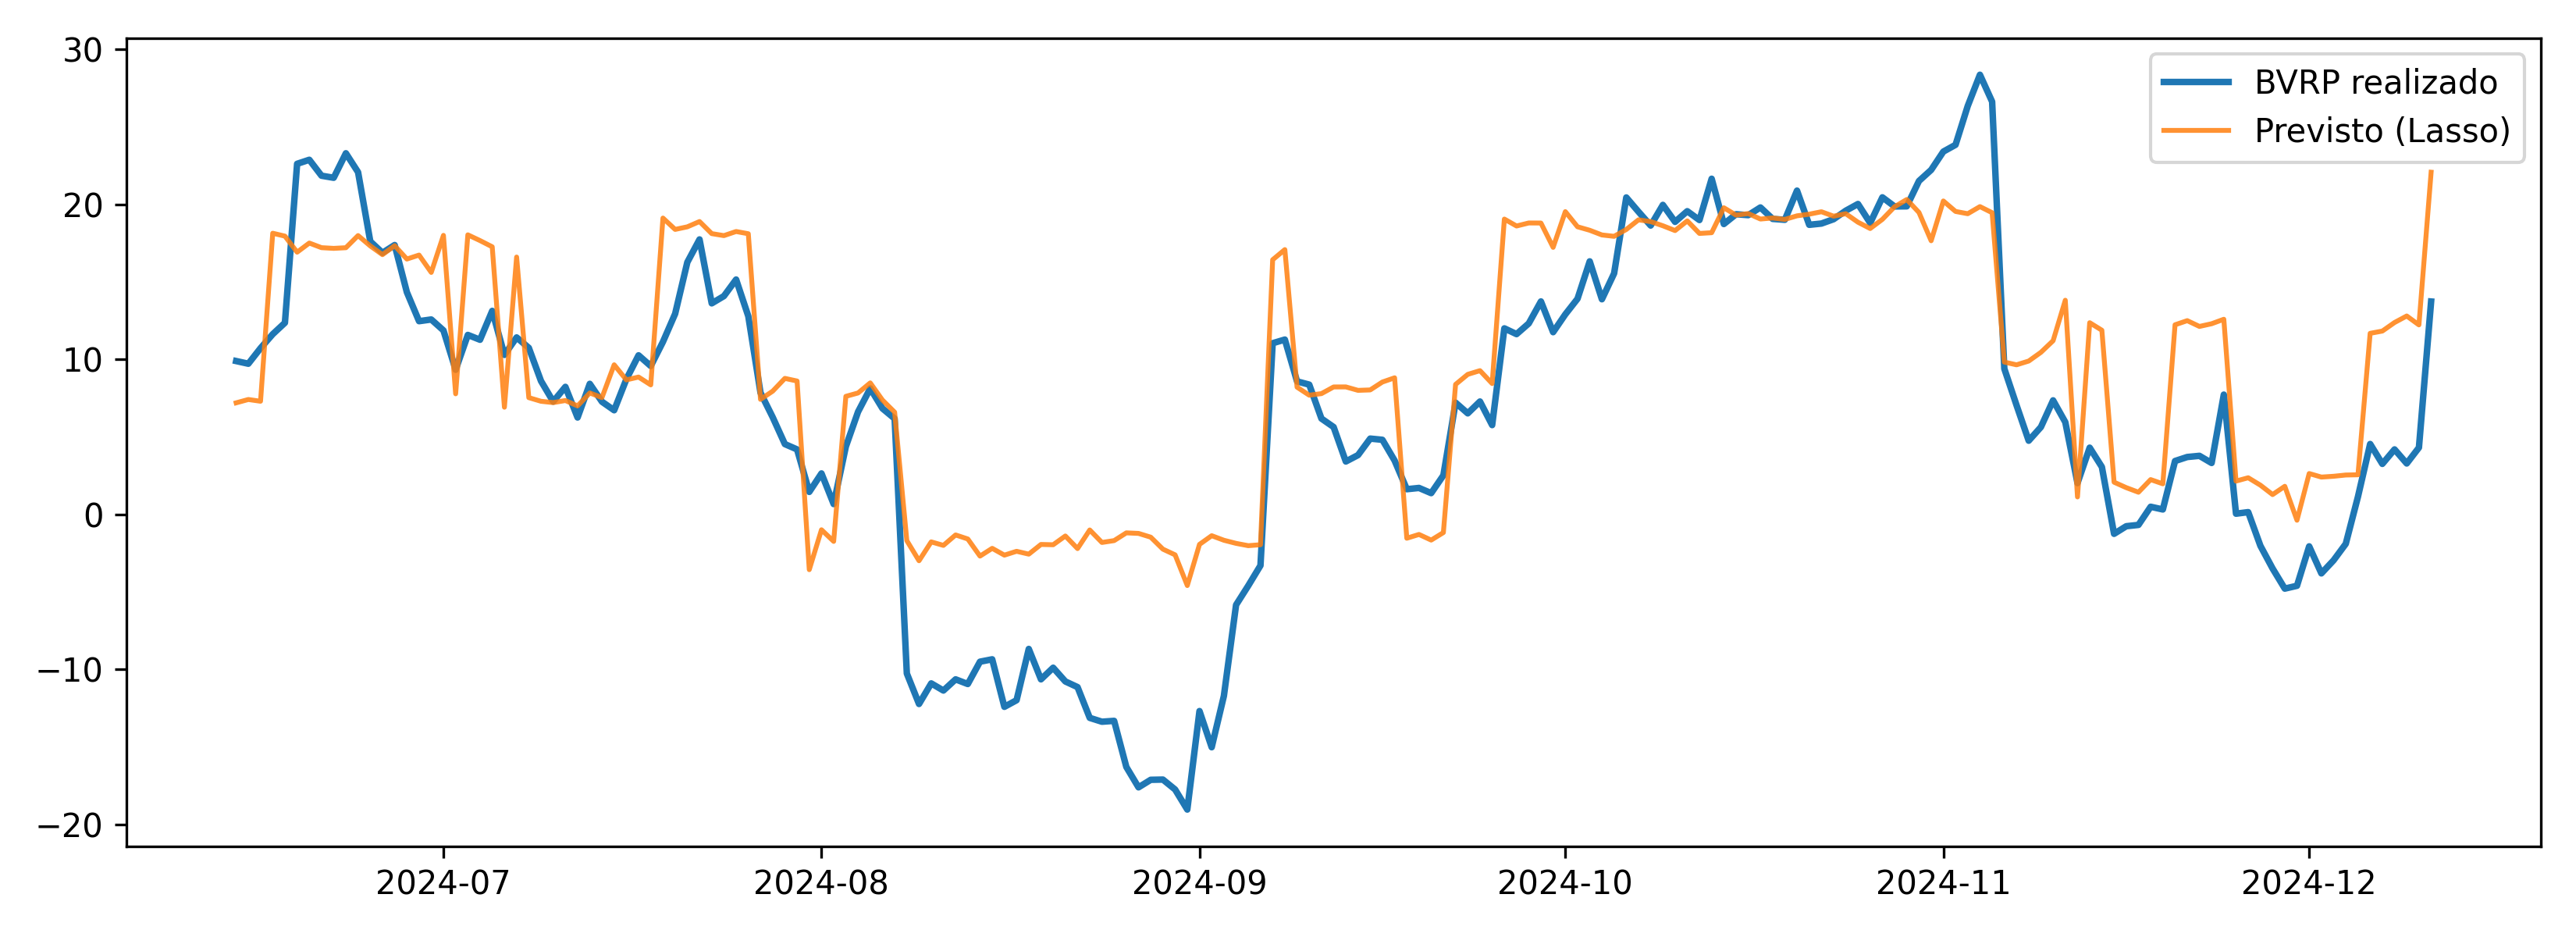
\includegraphics[width=0.9\textwidth]{figs/cap8/fig_cap8_oos_prediction.png}
\caption{Previsão fora da amostra do Prêmio de Risco de Volatilidade do Bitcoin.}
\label{fig:cap8_oos_prediction}
\end{figure}

\subsection{Comparação entre Modelos}
\label{sec:cap8_comparacao}

A hierarquia de desempenho sugere que parte relevante da previsibilidade do BVRP
decorre de relações relativamente estáveis e aproximadamente lineares entre o prêmio
e variáveis associadas à dinâmica recente de volatilidade e do próprio BVRP.
Isso é consistente com a presença de persistência temporal e com o fato de que o
prêmio é construído a partir de componentes (IV e RV) que exibem memória e regimes.

Modelos baseados em árvores e \textit{boosting} superam baselines fracos em muitos
cenários, indicando a presença de não linearidades e interações. Contudo, quando
comparados a baselines fortes e a modelos lineares parcimoniosos, seus ganhos fora
da amostra tendem a ser limitados, sugerindo que a contribuição marginal de
complexidade pode ser pequena na amostra analisada.

\subsection{Implicações Econômicas}
\label{sec:cap8_implicacoes}

As previsões do BVRP podem ser interpretadas como um insumo adicional para alocação
dinâmica de risco. Valores previstos elevados do prêmio sugerem ambientes em que a
compensação esperada por carregar risco de volatilidade é maior, possivelmente
associados a períodos de estresse e maior aversão ao risco. Em contraste, previsões
baixas podem sinalizar ambientes de menor atratividade do prêmio, nos quais a
exposição condicional pode ser menos eficiente.

Contudo, a evidência empírica sugere cautela: (i) a previsibilidade incremental além
da persistência pode ser moderada; (ii) resultados podem depender do período amostral;
e (iii) ganhos econômicos líquidos exigem considerar custos de transação, fricções e
robustez a mudanças de regime. Em conjunto, os achados são compatíveis com um ambiente
de eficiência parcial no mercado de opções de Bitcoin, no qual parte do prêmio é
previsível, porém difícil de explorar de forma robusta com modelos excessivamente
complexos.

\section{Análises de Robustez}
\label{sec:cap8_robustez}

Análises adicionais indicam que os resultados são qualitativamente robustos a variações
razoáveis na divisão temporal (treino/validação/teste), na seleção de variáveis explicativas
e em hiperparâmetros dos modelos. Em particular, a ordem relativa entre classes de modelos
tende a permanecer estável: baselines fortes de persistência e modelos lineares
parcimoniosos figuram entre os melhores desempenhos fora da amostra, enquanto modelos mais
flexíveis apresentam ganhos marginais e maior sensibilidade a especificações.

Essas evidências reforçam a interpretação de que a previsibilidade do BVRP é real, porém
em grande medida associada a componentes persistentes e à dinâmica de volatilidade, o que
impõe limites à exploração econômica via modelos altamente complexos.
